\chapter{Formalismo di Lagrange}
   Ci poniamo ora l'obiettivo di determinare l'equazione del moto di un sistema meccanico sottoposto a vincoli. Un vincolo è una condizione sulle coordinate o sulle velocità dei punti materiali che compongono il sistema meccanico. Chiamiamo vincoli \emph{bilateri} o bilaterali quelli che possono essere espressi tramite una relazione di uguaglianza del tipo:
   \begin{equation}
       \phi(x_1,\dots, x_{3n},\dot{x}_1,\dots, \dot{x}_{3n},t) = 0.
   \end{equation}
   Chiamiamo \emph{unilateri} o unilaterali i vincoli che sono invece riconducibili ad una relazione di disuguaglianza:
    \begin{equation}
       \phi(x_1,\dots, x_{3n},\dot{x}_1,\dots, \dot{x}_{3n},t) \leq 0.
   \end{equation}
   Un esempio di vincolo bilatero è una sbarra rigida che unisce due punti materiali
    $\x,\,\y$. Se la sbarra è di lunghezza $l$, 
    allora la distanza tra i due punti deve essere
    esattamente uguale ad $l$ ad ogni tempo $t$, dunque il vincolo sarà descritto dall'equazione
   \begin{equation}
       \|\x-\y\|=l \iff (x_1-y_1)^2 + (x_2-y_2)^2+(x_3-y_3)^2 -l^2 = 0.
   \end{equation}
   un vincolo unilatero è invece una corda di lunghezza $l$, che impedisce ai due punti $\x,\,\y$ di avere una distanza maggiore di $l$, ma permette che la distanza sia anche inferiore:
   \begin{equation}
       \|\x-\y\| \leq l \iff  (x_1-y_1)^2 + (x_2-y_2)^2+(x_3-y_3)^2 -l ^2\leq 0.
   \end{equation}
   Un vincolo $\phi$ è detto \emph{olonomo} se non dipende dalle velocità $\dot{x}_1,\dots,\dot{x}_{3n}$, mentre è detto \emph{anolonomo} se ne dipende. È detto reonomo se dipende dal tempo, scleronomo se non ne dipende\footnote{Rheo=scorrere, skleros=rigido, olos=intero.}.

   Quando si studia un sistema meccanico si deve affrontare un sistema di $3n$ equazioni differenziali ordinarie del secondo ordine, ovvero l'equazione di Newton proiettata su ogni componente di ogni punto materiale, più $m$ equazioni di vincolo\footnote{se $m=0$ allora il sistema è detto "libero", altrimenti "vincolato"}. Per i nostri scopi supporremo sempre che i vincoli siano olonomi e bilateri, dunque il sistema sarà del tipo
   \begin{equation}
       \begin{cases}
           m_1 \ddot{x}_1 = f_1 + R_1\\
           \vdots\\
           m_n \ddot{x}_{3n} = f_{3n} + R_{3n}\\
           \phi_1(x_1,\dots,x_{3n},t) = 0\\
           \vdots \\
           \phi_m(x_1,\dots,x_{3n},t) = 0
       \end{cases},
       \label{sistema di newton vincolato}
   \end{equation}
   dove si noterà che abbiamo separato la forza a cui le $x_k$ sono soggette in due contributi: $R_k$ è la forza dovuta al vincolo, detta \emph{reazione vincolare}, mentre $f_k$ è la forza complessiva dovuta a tutti gli altri contributi. In generale è possibile conoscere le $f_k$ grazie allo studio della situazione fisica, mentre le forze di vincolo sono generalmente sconosciute. Questo vuol dire che i vincoli complicano il problema rispetto al caso del sistema libero, in quanto introducono $3n$ incognite aggiuntive, una per ciascuna componente $R_k$ delle reazioni vincolari. In totale le incognite sono $3n+3n=6n$, mentre le equazioni sono $3n+m$. Poiché la norma è che i vincoli siano in numero minore delle componenti ($m<3n$), il sistema è in generale sotto determinato. Ci poniamo ora il problema di descrivere il sistema \ref{sistema di newton vincolato} in modo agevole, di studiarlo e di determinare le condizioni sotto cui potrebbe essere possibile uguagliare il numero di incognite e di equazioni. Prima di farlo osserviamo che il sistema \ref{sistema di newton vincolato} può essere scritto in forma vettoriale come
   \begin{equation}
   \begin{cases}
       \underline{m}\,\underline{\ddot{X}} = \underline{F}+\underline{R}\\
       \Phi = 0
    \end{cases}    
   \end{equation}
   dove $\underline{m},\underline{\ddot{X}},\,\underline{F},\,\underline{R} \in \R^{3n}$, $\Phi: \R^{3n+1} \to \R^m$. Chiameremo $\Phi$ funzione rappresentatrice dei vincoli e $\R^{3n}$ spazio delle configurazioni.
   
   \section{Varietà differenziabili, coordinate lagrangiane}
    La funzione rappresentatrice dei vincoli individua un sottoinsieme di $\R^{3n}$ formato dai punti che soddisfano il vincolo ad un dato istante:
    \begin{equation}
        M = \{(x_1,\dots,x_{3n}) \in \R^{3n}: \Phi(x_1,\dots,x_{3n},t ) = 0\,\forall t\} = M_t.
    \end{equation}
    Per esempio il vincolo
    \begin{equation}
        \phi(x,y) = x^2+y^2-R^2 = 0
    \end{equation}
    individua l'insieme
    \begin{equation}
        C = \{(x,y)\in \R^2 : x^2+y^2=R^2\},
    \end{equation}
    che è una circonferenza centrata nell'origine e di raggio $R$. Invece $x^2+y^2-t^2=0$ rappresenta una circonferenza con raggio crescente nel tempo, dunque l'insieme dei punti che soddisfano il vincolo è funzione del tempo $C=C(t)$ e lo possiamo immaginare come una circonferenza che si espande nel piano $\R^2$.
    
    Consideriamo ora lo jacobiano della funzione $\Phi$:
    \begin{equation}
        J_\Phi = 
        \begin{bmatrix}
            \frac{\partial \phi_1}{\partial x_1}&\dots& \frac{\partial \phi_1}{\partial x_{3n}}&\frac{\partial \phi_1}{\partial t}\\
            \vdots&\dots&\dots&\vdots\\
            \frac{\partial \phi_m}{\partial x_1}&\dots&\frac{\partial \phi_m}{\partial x_{3n}}
            &\frac{\partial \phi_m}{\partial t}
        \end{bmatrix} = \begin{bmatrix}
            \nabla \phi_1\\
            \vdots\\
            \nabla \phi_m
        \end{bmatrix}
    \end{equation}
    Supponiamo che $\Phi$ sia di classe $C^1$ almeno, in modo che lo jacobiano sia una matrice di funzioni continue. Lo jacobiano è una matrice $m \times (3n+1)$ e, essendo $m<3n$, il suo rango vale al massimo $m$. Se la sottomatrice
    \begin{equation}
        D_{k,\,j} = \frac{\del \phi_k}{\del x_j}
    \end{equation}
    ha rango $m$ allora esisteranno $m$ colonne linearmente indipendenti, che possiamo supporre essere, a meno di permutazioni degli indici, le colonne $1,\dots,m$. Allora possiamo decomporre lo jacobiano di $\Phi$ in due sottomatrici:  
   \begin{equation}
        JF=\left[\begin{array}{ccc|cccc}
   \frac{\partial \phi_1}{\partial x_1}&\dots& \frac{\partial \phi_1}{\partial x_{m}}&\frac{\partial \phi_1}{\partial x_{m+1}}&\dots&\frac{\partial \phi_1}{\partial x_{3n}}&\frac{\partial \phi_1}{\partial t}\\
            \vdots&\ddots&\vdots&\vdots&\ddots&\vdots&\vdots\\
            \frac{\partial \phi_m}{\partial x_1}&\dots&\frac{\partial \phi_m}{\partial x_{m}}&\frac{\partial \phi_m}{\partial x_{m+1}}&\dots&\frac{\partial \phi_1}{\partial x_{3n}}
            &\frac{\partial \phi_m}{\partial t}
\end{array}\right]=\begin{bmatrix}
    X | Y
\end{bmatrix},
    \end{equation}
    in cui $X$ è una matrice invertibile. Il teorema di Dini assicura quindi l'esistenza locale di una funzione $g(x_{m+1},\dots,x_{3n},\,t): \R^{3n-m+1} \to \R^m$ che permette di parametrizzare il luogo $M(t) = \{\Phi = 0\}$ in funzione delle sole coordinate $x_{m+1},\dots,x_{3n}$ e del tempo $t$. In altre parole calcolare $g(x_{m+1},\dots,x_{3n},\,t)$ restituisce le coordinate $x_1,\dots,x_m$:
    \begin{equation}
        (x_1,\dots,x_m) = g(x_{m+1},\dots,x_{3n},\,t),
    \end{equation}
    e vale
    \begin{equation}
        \phi[g(x_{m+1},\dots,x_{3n},\,t),x_{m+1},\dots,x_{3n},\,t] \equiv 0,
    \end{equation}
    ovvero $(g(x_{m+1},\dots,x_{3n},\,t),\,x_{m+1},\dots,\,x_{3n}) \in M$ $\forall t$.
    
    In soldoni quello che stiamo dicendo è che se la funzione rappresentatrice dei vincoli è sufficientemente regolare --- ovvero è di classe $C^1$ e il rango della sottomatrice $D$ è massimo --- allora quando i punti materiali rispettano il vincolo non ho bisogno di tutte le $3n$ coordinate per dire dove si trovano gli $n$ punti, bensì ho bisogno solamente di $3n-m$ coordinate perché, date $x_{m+1},\dots,x_{3n}$, posso ricavare le coordinate $x_1,\dots,x_m$ in funzione del tempo calcolando la funzione $g$ al tempo $t$. Questo vuol dire che il sistema ha $3n-m$ gradi di libertà, in quanto la posizione dei punti è descritta da $3n-m$ incognite scalari. Tutto questo argomento non è altro che la formalizzazione di un idea intuitiva: un sistema di $n$ punti materiali soggetto a $m$ vincoli bilateri olonomi non ha $3n$ gradi di libertà, ne ha $3n-m$, perché i vincoli limitano i gradi di libertà. Quando $\Phi$ è sufficientemente regolare l'insieme di vincolo $M$ prende il nome di \emph{varietà differenziabile}. Una varietà differenziabile è $l$ dimensionale se la funzione $g$ che la parametrizza è funzione di $l$ variabili indipendenti. La varietà descritta sopra sarebbe quindi $3n-m$ dimensionale.
     
    Per capire come funziona il processo consideriamo ad esempio il vincolo 
    \begin{equation}
        \phi(x,y) = x^2+y^2-R^2=0.
    \end{equation}
    Lo jacobiano di $\phi$ è una matrice $1\times 2$, che coincide con il gradiente della funzione:
    \begin{equation}
        J_\phi = \nabla \phi = \left(\frac{\del \phi}{\del x},\,\frac{\del \phi}{\del y}\right) = (2x,2y)
    \end{equation}
    il rango della matrice è massimo se è uguale a $1$. Affinché questo sia soddisfatto deve essere $x,\,y \neq 0$, che è sempre vero per $(x,y) \neq(0,0)$, ma il luogo dei punti individuato dal vincolo è una circonferenza di centro $(0,0)$ e raggio $R>0$, dunque il rango è sempre massimo. Per quanto detto sopra dovrebbe esistere una funzione $g(x)$ che parametrizza il vincolo. La possiamo trovare esplicitamente:
    \begin{equation}
        x^2+y^2-R^2 = 0 \implies y = \pm \sqrt{R^2-x^2} = \pm g(x).
    \end{equation}
    Vediamo che effettivamente i punti $x,\,g(x)$ appartengono sempre al vincolo:
    \begin{equation}
        \phi(x, \pm g(x)) = x^2 + R^2-x^2 -R^2 \equiv 0,
    \end{equation}
    dunque il sistema è effettivamente a un solo grado di libertà. La presenza del $\pm$ è dovuta al fatto che $+g$ parametrizza la semicirconferenza superiore e $-g$ quella inferiore. A questo punto posso anche vedere che poiché $x\in[-R,\,R]$ posso parametrizzare $x$ in funzione di un parametro $\theta$ in modo che 
    \begin{equation}
        x= R\cos \theta,
    \end{equation}
     così anche 
     \begin{equation}
     y = \sqrt{R^2-R^2\cos^2\theta} = R\sin\theta,
     \end{equation}
     dunque c'è libertà nella scelta della parametrizzazione 
     del vincolo. In generale, data una funzione 
     $g(x_{m+1},\dots,\,x_{3n})$, posso trovare 
     $l=3n-m$ parametri $q_1,\dots, q_l$ in modo da trasformare $g$ 
     in $g(q_1,\dots,q_l)$. 
     La libertà nella scelta di $q_1,\dots, q_l$ ha
      fatto guadagnare a questi parametri il nome di 
      \emph{coordinate generalizzate}. Per motivi storici 
      sono anche note come \emph{coordinate lagrangiane}.

    \begin{example}
        \textbf{La pallina e il cono ellittico}\\
        Il luogo dei punti che costituisce la superficie di un cono a base ellittica è descritto dal vincolo
        \begin{equation}
            \phi(x,y,z) = (x/a)^2+(y/b)^2 - z^2 = 0
        \end{equation}
        \begin{center}
        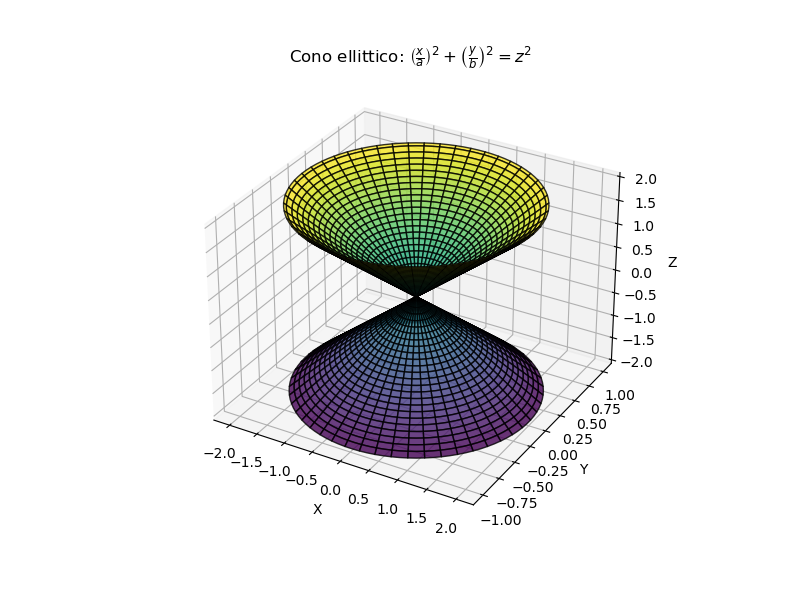
\includegraphics[width=0.8\linewidth]{img/conoEllittico.png}
        \end{center}
        Procedendo come prima possiamo invertire la funzione usando $x,y$ come parametri:
        \begin{equation}
            z = \pm \sqrt{(x/a)^2+(y/b)^2}.
        \end{equation}
        $z_+$ parametrizza il cono con la punta verso il basso, $z_-$ quello con la punta verso l'alto. Supponiamo ora di avere un problema meccanico in cui una pallina, soggetta alla forza di gravità, è obbligata a rimanere ancorata al cono con la punta verso il basso. Il sistema del moto sarebbe
        \begin{equation}
        \begin{cases}
            m\ddot{x} = R_x\\
            m\ddot{y} = R_y \\
            m\ddot{z} = R_z -mg \\
            \phi(x,y,z) = 0
        \end{cases}
        \end{equation}
        l'equazione di vincolo permette di esprimere $z$ in funzione di $x,y$, e questa osservazione permette di scrivere il nuovo sistema del moto come
        \begin{equation}
            \begin{cases}
            m\ddot{x} = R_x\\
            m\ddot{y} = R_y \\
            m \frac{\de^2}{\de t^2} \sqrt{(x(t)/a)^2+(y(t)/b)^2} = R_z -mg
            \end{cases}
        \end{equation}
        che ha 5 incognite $x,y, R_x,R_y,R_z$ e $3$ equazioni: il sistema è ancora sotto determinato.
        Questo esempio, come anche il precedente, permettono di capire che in un certo senso l'esistenza della funzione $g$ permette di vedere $M$ come il grafico di $g$.
    \end{example}
    \subsection{Fibrato tangente e fibrato ortogonale}
    Discutiamo le proprietà geometriche della varietà differenziabili. Consideriamo una curva $\q(\alpha): \R \to \R^l,\, \q(\alpha) = (q_1(\alpha),\dots, q_l(\alpha)).$ Posso comporre $\q(\alpha)$ con la funzione $g$ che parametrizza $M$. In questo modo ottengo
    \begin{equation}
        \x(\alpha) \equiv (x_1,\dots,\,x_{3n}) = (\g(\q(\alpha)),x_{m+1},\dots,x_{3n})
    \end{equation}
    per cui $x_k = x_k(q_1,\dots,\,q_l),\, \forall k \in \{1,\dots,3n\}$, e 
    \begin{equation}
       \boldsymbol{\tau} = \frac{\de \x}{\de \alpha} = \sum_{k=1}^l \frac{\del \x}{\del q_k} q'_k(\alpha)\,.
        \label{var_temp}
    \end{equation}
    Quando componiamo $\g$ e $\q$ stiamo trasportando la curva dallo spazio vettoriale euclideo in cui risiede il vettore $\q$ allo spazio $M$ della varietà differenziabile:
    \begin{equation}
        \q: \R \to \R^l,\implies\,\x = (g(\q),x_{m+1},\dots,x_{3n}): \R \to M
    \end{equation}
    Sappiamo dall'analisi che quando deriviamo una curva $\q(\alpha)$ otteniamo un vettore $\q'(\alpha)$ tangente alla curva stessa. Quando la curva viene trasportata sulla varietà otteniamo una curva sulla varietà, e anche la derivata di questa curva sarà tangente alla curva ma, essendo stavolta la curva contenuta nella varietà, $\x'(\alpha)$ sarà tangente anche alla varietà. Possiamo ora definire altre curve, $\boldsymbol{\xi}(\alpha),\,\boldsymbol{\psi}(\alpha),\dots$, e trasportare ciascuna di queste su $M$. Derivando otterremo altri vettori tangenti ad $M$, che saranno di forma simile alla $\boldsymbol{\tau}$ della \ref{var_temp}, ma in cui gli scalari $q'_k(\alpha)$ diventeranno $\xi_k'(\alpha),\, \psi_k'(\alpha),\dots$. La derivata di $\x$ rispetto a $q_k$ è la stessa cosa della derivata di $\x$ rispetto a $\xi_k$ in quanto si tratta in entrambi i casi di una notazione per indicare la derivata rispetto alla $k$-esima entrata
    \begin{equation}
        \frac{\del \x}{\del q_k}=\frac{\del \x}{\del \xi_k} = \del_k \x,
    \end{equation}
    Vediamo quindi che qualsiasi vettore $\boldsymbol{\tau}$ tangente a $M$ può essere espresso come combinazione lineare degli $l$ vettori
    \begin{equation}
        \frac{\del \x}{\del q_1},\dots,\, \frac{\del \x}{\del q_l},
    \end{equation}
    il che li rende un set di generatori dello \emph{spazio tangente}, che sarebbe lo spazio vettoriale 
    \begin{equation}
    T_xM_t = \{\boldsymbol{\tau}\in \R^{3n}: \boldsymbol{\tau}\,\mathrm{e'\,tangente\,a\,M\,nel\,punto}\,x \in M\}.
    \end{equation}
    
   La regolarità richiesta da $g$ assicura che i vettori $\partial_k \x$ siano linearmente indipendenti, consentendo di chiamarli \emph{base dello spazio tangente}. Questi vettori sono detti \emph{velocità virtuali} perché, se parametrizziamo $\q$ in funzione del tempo e consideriamo che $g$ è funzione del tempo (come ricorda il pedice $t$ che mettiamo a $M$), otteniamo che 
    \begin{equation}
        \dot{\x} = \sum_k \frac{\del \x}{\del q_k} \dot{q}_k + \frac{\del \x}{\del t},
    \end{equation}
    per cui la velocità effettiva è somma della velocità virtuale e della velocità di trascinamento $\del_t \x$ dovuta alla dipendenza di $M$ dal tempo. La velocità virtuale deve il suo nome al fatto che sarebbe la velocità del punto materiale se il vincolo fosse fermo nel tempo.
    
    Definiamo \emph{Fibrato tangente} l'insieme
    \begin{equation}
        TM_t = \bigcup_{x\in M} T_x M_t
    \end{equation}
    Lo spazio $T_xM_t$ è $l$-dimensionale perché ammette base composta da $l$ vettori. Essendo $l=3n-m$ ci aspettiamo che il suo complemento ortogonale $(T_xM_t)^\perp$ abbia dimensione $m$. 

    Per ragionare sullo spazio ortogonale a $M$ vediamo che, essendo $\x(\alpha) \in M$ e $\Phi=0\, \forall \x \in M$, allora $\Phi$ è costante sulla curva, per cui la sua derivata rispetto ad $\alpha$ è identicamente nulla:
    \begin{equation}
        0 \equiv \Phi(\x(\alpha)) \implies \frac{\de \Phi}{\de \alpha} = J_\Phi \frac{\de \x}{\de \alpha} = 0 .
    \end{equation}
    Osserviamo che il prodotto è ben definito in quanto $\x$ è un vettore con $m$ componenti e $J_\Phi$ ha $m$ righe.
    Se prendiamo $\q = (\alpha,0\,\dots, 0)$ allora il prodotto tra lo jacobiano della funzione rappresentatrice dei vincoli e il vettore velocità diventa il prodotto tra lo jacobiano e il primo elemento della base dello spazio tangente:
   \begin{equation}
       0 = J_\Phi \frac{\de \x}{\de \alpha} = J_\Phi \frac{\del \x}{\del q_1} = \begin{bmatrix}
           \frac{\partial \phi_1}{\partial x_1}&\dots& \frac{\partial \phi_1}{\partial x_{3n}}\\
            \vdots&\dots&\vdots\\
            \frac{\partial \phi_m}{\partial x_1}&\dots&\frac{\partial \phi_m}{\partial x_{3n}}            
       \end{bmatrix}
       \begin{bmatrix}
           \frac{\del x_1}{\del q_1}\\
           \vdots\\
           \frac{\del x_m}{\del q_1}
       \end{bmatrix} = \begin{bmatrix}
           \braket{\nabla\phi_1 |\frac{\del \x}{\del q_1}}\\
           \vdots \\
        \braket{\nabla \phi_m |\frac{\del \x}{\del q_1}}\,.
       \end{bmatrix}
   \end{equation}
    Affinché l'uguaglianza sia rispettata deve essere nullo il prodotto scalare tra $\nabla \phi_k$ e il primo vettore della base $\forall k \in \{1,\dots,m\}$, ovvero i vettori $\nabla \phi_1, \dots, \nabla \phi_m$ sono tutti ortogonali a $\del_1 \x$. Scegliendo la curva $\q = (0, \alpha,0,\dots,0)$ si troverà analogamente che i gradienti sono ortogonali a $\del_2 \x$, dunque si dovrà concludere che
    \begin{equation}
        \nabla \phi_k \in (T_xM_t)^\perp \,\forall k \in \{1,\dots,m\}.
    \end{equation}
    Essi formano una base dello spazio ortogonale perché sono $m$ e sono linearmente indipendenti, in quanto il rango della matrice $D$ è $m$ e quindi tutte le righe che la compongono, che sono per l'appunto i gradienti dei vincoli, devono essere linearmente indipendenti. Lo spazio ha dimensione al più $m$ e quindi è tutto dimostrato. Definiamo similmente a prima il \emph{fibrato ortogonale} come 
    \begin{equation}
        (TM_t)^\perp = \bigcup_{x\in M} (T_xM_t)^\perp
    \end{equation}
    
    \section{Principio dei lavori virtuali, equazioni di Eulero-Lagrange}
    La geometria dei vincoli suggerisce la condizione affinché il sistema \ref{sistema di newton vincolato} abbia sempre lo stesso numero di incognite e di equazioni. Basta richiedere che il vettore $\underline{R}$, che in generale appartiene allo spazio delle configurazioni $\R^{3n}$, appartenga in ogni istante $t$ al sottospazio di $\R^{3n}$ costituito dallo spazio ortogonale di $M$, $(T_xM_t)^\perp.$ In tal caso infatti si avrebbe che $\underline{R}$ è esprimibile come combinazione lineare dei gradienti dei vincoli, ovvero
    \begin{equation}
        \underline{R} = \sum_{k=1}^m \lambda_k \nabla \phi_k,
    \end{equation}
    dunque le incognite scalari del sistema, che erano in principio $3n+3n=6n$, diventano $3n+m$: $3n$ sono le coordinate dei punti, $m$ sono i fattori $\lambda_k$ che determinano univocamente $\underline{R}$ e quindi ciascuna delle sue componenti $R_1 \dots, R_{3n}$. In altre parole stiamo richiedendo che il prodotto scalare tra $\underline{R}$ e qualsiasi vettore velocità virtuale $\tau$ sia nullo. Esprimendo $R_k = m_k \ddot{x}_k -f_k$, possiamo scrivere la condizione come
   \begin{equation}
       \sum_{k=1}^{3n} (m_k \ddot{x}_k - f_k) \tau_k = 0,
   \end{equation}
   detto principio di D'Alembert. Un vincolo che rispetti il principio di D'Alembert è detto vincolo ideale o liscio. Per un tale sistema il moto è dato dal sistema
   \begin{equation}
       \begin{cases}
           m_k \ddot{x}_k = f_k + \left[\sum_{i=1}^n \lambda_i \nabla \phi_i\right]_k \\
           \Phi = 0
       \end{cases}.
   \end{equation}
   L'equazione $ m_k \ddot{x}_k = f_k + \left[\sum_{i=1}^n \lambda_i \nabla \phi_i\right]_k$ è detta \emph{equazione di Eulero-Lagrange in prima forma.}

   Possiamo fare di più. Abbiamo visto che in realtà non sono necessarie $3n$ coordinate per determinare lo stato del sistema, bensì bastano le sole $l=3n-m$ coordinate lagrangiane. Il nostro nuovo obiettivo è quindi trasformare il sistema delle $3n$ equazioni del moto in un sistema di $l$ equazioni scritte per le coordinate $q_1, \dots,\,q_l$:

    \begin{theorem}
    \textbf{Equazioni di Eulero-Lagrange, II forma.}\\
    Sia dato un sistema meccanico di $n$ punti materiali, di coordinate $x_1, \dots, x_{3n}$, ed $m$ vincoli bilateri olonomi ideali $\phi_1,\dots,\phi_m$, sottoposto a forze conservative di componenti $f_1,\dots,f_{3n}$ riconducibili ad un potenziale $V$. Supponiamo inoltre che i vincoli siano sufficientemente regolari da permettere di ricondurre le posizioni dei punti alle coordinate lagrangiane $q_1,\dots,q_l$. Allora il moto è determinato dalle equazioni
    \begin{equation}
        \deriv \frac{\del \lag}{\del \dot{q}_k} - \frac{\del \lag}{\del q_k} = 0,\, \forall k \in \{1,\dots,m\}
    \end{equation}
    dove $\lag(\q,\dot{\q},t)$ è detta \emph{Lagrangiana} del sistema ed è definita da
    \begin{equation}
        \lag(\q,\dot{\q},t) = T(\q,\dot{\q},t)-V(\q),
    \end{equation}
    con $T$ l'energia cinetica del sistema.
    \end{theorem}
    \begin{proof}
    Per dimostrare il teorema è fondamentale osservare che
    \begin{equation}
        \dot{x}_k = \deriv x_k(q_1,\dots,q_l, t) = \sum_{j=1}^l \frac{\del x_k}{\del q_j}\dot{q}_j + \frac{\del x_k}{\del t}
    \end{equation}
    per cui
    \begin{equation}
        \frac{\del \dot{x}_k}{\del \dot{q}_j} = \frac{\del x_k}{\del q_j},
    \end{equation}
    perché $x_k$ non dipende dalle velocità e quindi $\del_t x_k$ si annulla quando è derivata rispetto a $\dot{q}_j$. Osservato questo possiamo iniziare a dimostrare l'equazione di Eulero-Lagrange per verifica diretta:
    \begin{equation}
        \frac{\del}{\del \dot{q}_j} \lag = \frac{\del}{\del \dot{q}_j} (T-V) = \frac{\del}{\del \dot{q}_j}T,
    \end{equation}
    perché $V$ non dipende dalle velocità. D'altra parte $T = \frac{1}{2}\sum_{k=1}^{3n}m_k\dot{x}_k^2$ allora quando derivo ottengo 
    \begin{equation}
        \frac{\del}{\del \dot{q}_j}T = \sum_{k=1}^{3n} m_k \dot{x}_k \frac{\del \dot{x}_k}{\del \dot{q}_j} = \sum_{k=1}^{3n} m_k \dot{x}_k \frac{\del x_k}{\del q_j}.
    \end{equation}
    Derivando rispetto al tempo otteniamo
    \begin{equation}
        \deriv \frac{\del \lag}{\del \dot{q}_j} = \sum_{k=1}^{3n} m_k \ddot{x}_k \frac{\del x_k}{\del q_j} + m_k \dot{x}_k \frac{\del \dot{x}_k}{\del q_j}
    \end{equation}
    dove abbiamo scambiato la derivata rispetto al tempo e quella rispetto al $q_j$ per il teorema di Schwarz sulle derivate miste. Calcoliamo ora
    \begin{equation}
        \frac{\del \lag}{\del q_j} = \sum_{k=1}^{3n}m_k\dot{x}_k \frac{\del \dot{x}_k}{\del q_j} - \frac{\del V}{\del x_k}\frac{\del x_k}{\del q_j}
    \end{equation} 
    e sottraendo le due espressioni, troviamo 
    \begin{equation}
        \sum_{k=1}^{3n} m_k \ddot{x}_k \frac{\del x_k}{\del q_j} + m_k \dot{x}_k \frac{\del \dot{x}_k}{\del q_j} -\left[\sum_{k=1}^{3n}m_k\dot{x}_k \frac{\del \dot{x}_k}{\del q_j} - \frac{\del V}{\del x_k}\frac{\del x_k}{\del q_j}\right] 
    \end{equation}
    ovvero, riconoscendo la derivata di $V$ come la $k$-esima componente della forza :
    \begin{equation}
        \frac{\del V}{\del x_k} = -f_k
    \end{equation}
    si ottiene
    \begin{equation}
        \sum_{k=1}^{3n}(m_k\ddot{x}_k - f_k)\frac{\del x_k}{\del q_j},
    \end{equation}
    ma abbiamo detto che i vincoli sono lisci, dunque per definizione
    \begin{equation}
        \sum_{k=1}^{3n}(m_k\ddot{x}_k - f_k)\frac{\del x_k}{\del q_j}=0
    \end{equation}
    ovvero
    \begin{equation}
        \deriv \frac{\del \lag}{\del \dot{q}_j}-\frac{\del \lag}{\del q_j}=0
    \end{equation}
    \end{proof}
    Osserviamo che le equazioni di Eulero-Lagrange possono essere formulate anche per forze non conservative in modo assolutamente analogo:
   \begin{equation}
       \deriv \frac{\del T}{\del \dot{q}_j} - \frac{\del T}{\del q_j} = Q_j,
   \end{equation}
   con $Q_j = \sum_{i=1}^{3n} f_i \frac{\del x_i}{\del q_j}$. È facile verificare che questa formula è vera ripercorrendo i passaggi della dimostrazione precedente e variando solo quello in cui si sostituisce il potenziale. 

   \subsection{Esistenza e unicità della soluzione delle equazioni di Eulero-Lagrange}
   Ci chiediamo ora se le equazioni di Eulero-Lagrange siano sufficienti per determinare univocamente il moto, ossia se sia possibile applicargli il teorema di esistenza e unicità. Questo non è scontato perché a un primo sguardo le equazioni di Eulero-Lagrange coinvolgono derivate parziali e sono accoppiate in modo non banale, per cui non è ovvio che sia possibile ricondurle ad una forma del tipo $\ddot{\q} = F(\q,\,\dot{\q},\,t).$ 
   
   Per procedere in questo scopo scriviamo in modo più esplicito l'energia cinetica $T$ ricordando che $\dot{x_i} = \sum_k \del_kx_i \dot{q}_k + \del_t x_i$ e sostituendo:   
    \begin{equation}
        T = \sum_{i=1}^{3n} \frac{m_i}{2} \dot{x}_i^2 = \sum_{i=1}^{3n} \frac{m_i}{2} \left[\sum_{k=1}^l \frac{\partial x_i}{\partial q_k}\dot{q}_k + \frac{\partial x_i}{\partial t}\right]^2
        \label{T 1}
    \end{equation}
    
    svolgendo il quadrato otteniamo
    \begin{equation}
    \left[\sum_{k=1}^l \frac{\partial x_i}{\partial q_k}\dot{q}_k + \frac{\partial x_i}{\partial t}\right]^2 = \left[\sum_{k=1}^l \frac{\partial x_i}{\partial q_k}\dot{q}_k\right]^2 +
    2\left[\sum_{k=1}^l \frac{\partial x_i}{\partial q_k}\dot{q}_k\frac{\partial x_i}{\partial t}\right]+   
    \left[\frac{\partial x_i}{\partial t}\right]^2,
    \end{equation}
    per cui $T=T_1+T_2+T_3$, dove $T_1$ è quadratico in $\dot{q}_k$, $T_2$ è lineare in $\dot{q}_k$ e $T_3$ è costante rispetto a $\dot{q}_k$. Possiamo scrivere il quadrato della sommatoria attraverso una sommatoria su due indici:
    \begin{equation}
         \left[\sum_{k=1}^l \frac{\partial x_i}{\partial q_k}\dot{q}_k\right]^2 = \sum_{j,k=1}^{l} \frac{\partial x_i}{\partial q_k}\frac{\partial x_i}{\partial q_j}\dot{q}_k\dot{q}_j
         \label{quadrato della sommatoria}
    \end{equation}
    per cui $T$ può essere esplicitata come
    \begin{equation}
        T = \sum_{i=1}^{3n}\frac{m_i}{2}\left[\sum_{j,k=1}^{l} \frac{\partial x_i}{\partial q_k}\frac{\partial x_i}{\partial q_j}\dot{q}_k\dot{q}_j\right]+ \sum_{i=1}^{3n}m_i\left[\sum_{k=1}^l \frac{\partial x_i}{\partial q_k}\dot{q}_k\frac{\partial x_i}{\partial t}\right]+ \sum_{i=1}^{3n}\frac{m_i}{2}\left[\frac{\partial x_i}{\partial t}\right]^2.
    \end{equation}
    nella prima sommatoria possiamo vedere una forma quadratica di una matrice $l\times l$ che chiamiamo $A$:
    \begin{equation}
    A=
            \begin{bmatrix}
                \sum_{i=1}^{3n}m_i\frac{\partial x_i}{\partial q_1}\frac{\partial x_i}{\partial q_2}& \dots & \sum_{i=1}^{3n}m_i\frac{\partial x_i}{\partial q_1}\frac{\partial x_i}{\partial q_l}\\
                \vdots& \ddots &\vdots\\ 
                \sum_{i=1}^{3n}m_i\frac{\partial x_i}{\partial q_l}\frac{\partial x_i}{\partial q_1} & \dots& \sum_{i=1}^{3n}m_i\frac{\partial x_i}{\partial q_l}\frac{\partial x_i}{\partial q_l}
        \end{bmatrix} = \left(\sum_{i=1}^{3n} m_i \frac{\del x_i}{\del q_k}\frac{\del {x_i}}{{\del q_{k'}}}\right)_{k,k'}
    \end{equation}
    Questo ci consente di scrivere $T_1 = \braket{\dot{\q}|A\dot{\q}}/2$. Le proprietà della matrice $A$ sono la chiave per dimostrare l'unicità della soluzione delle equazioni di Eulero-Lagrange e saranno utili anche quando introdurremo il Formalismo Hamiltoniano. Osserviamo in particolare che  $A$ è \textbf{definita positiva}, ovvero $\braket{\eta|A\eta}\geq0\,\forall \eta \in \R^{l}$ e $\braket{\eta|A\eta}=0 \iff \eta =0$. Per dimostrarlo vediamo che
    \begin{equation}
       \braket{\eta|A\eta} = \sum_{k,\,j=1}^l \eta_k\eta_j\sum_{i=1}^{3n}\frac{m_i}{2}\frac{\partial x_i}{\partial q_k}\frac{\partial x_i}{\partial q_j} =\sum_{i=1}^{3n}\frac{m_i}{2}\sum_{j,\,k=1}^l\frac{\partial x_i}{\partial q_k}\frac{\partial x_i}{\partial q_j} \eta_j \eta_k 
    \end{equation}
    ma, per quanto abbiamo visto nella \eqref{quadrato della sommatoria}, possiamo scrivere
    \begin{equation}
        \eta A\eta^t = \sum_{i=1}^{3n}\frac{m_i}{2}\left[\sum_{k=1}^l\frac{\partial x_i}{\partial q_k} \eta_k\right]^2,
    \end{equation}
    che è sempre $\geq0$ in quanto le masse $m_i$ sono strettamente positive. Il fatto che le masse siano non nulle implica che $\braket{\eta|A\eta}$ è nullo solo se si annulla
    \begin{equation}
        \sum_{k=1}^l\frac{\partial x_i}{\partial q_k} \eta_k
    \end{equation}
    $\forall i\in\{1,\dots,\,3n\}$, ma questa è l'i-esima componente una combinazione lineare dei vettori di una base, ovvero la base dello spazio tangente alla varietà dei vincoli, per cui è nulla $\forall\,i$ se e solo se $\eta=0,$ come volevasi dimostrare. $A$ è anche ovviamente simmetrica per la proprietà commutativa del prodotto. Le matrici simmetriche definite positive sono matrici rappresentative di prodotti scalari, per questo motivo la matrice $A$ è detta anche \emph{matrice di metrica cinetica.} Osserviamo anche che $A$ è simmetrica perché coincide con l'Hessiano di T fatto rispetto alle variabili $\dot{\q}$.
    che è una proprietà utile da sapere quando si vuole trovare $A$ nelle applicazioni\footnote{Per dimostrarlo ricordare che $\del_{\dot q}\dot{x}=\del_q x$}.
    Nella seconda sommatoria di $T$ posso vedere un prodotto scalare, tra il vettore
    \begin{equation}
        B = \left(\sum_{i=1}^{3n}m_i\frac{\partial x_i}{\partial q_1}\frac{\partial x_i}{\partial t},\dots,\sum_{i=1}^{3n}m_i\frac{\partial x_i}{\partial q_l}\frac{\partial x_i}{\partial t}\right)
    \end{equation}
    e il vettore $\dot{q}=(\dot{q}_1,\dots,\dot{q}_l)$ per cui, in ultimo,
    \begin{equation}
        T = \frac{1}{2}\braket{\dot{\q}|A\dot{\q}} + B \dot{\q} + T_3
    \end{equation}
    con 
    \begin{equation}
        T_3 = \sum_{i=1}^{3n}\frac{m_i}{2}\left[\frac{\partial x_i}{\partial t}\right]^2.
    \end{equation}
    Questo consente di scrivere una generica Lagrangiana come
    \begin{equation}
        \lag = \frac{1}{2}\braket{\dot{\q}|A\dot{\q}} + B \dot{\q} + T_3-V(\q),
    \end{equation}
    per cui le equazioni di Eulero-Lagrange saranno in generale
    \begin{equation}
       \begin{aligned}
           &\deriv \frac{\del \lag}{\del \dot{\q}} = \frac{\del{\lag}}{{\del \q}}\\
           &\deriv\left(A\dot{\q}+B\right) = f(\q,\dot{\q},t)\\
           &\dot{A}\dot{\q}+A\ddot{\q}+\dot{B} = f(\q,\dot{\q},t)\\
           &\ddot{\q} = A^{-1}\tilde{f}(\q,\,\dot{\q},\,t).
       \end{aligned}
    \end{equation}
    Il passaggio critico qui è chiaramente l'inversione di $A$, che non è affatto scontata. Tuttavia le matrici definite positive hanno anche ker banale, per cui sono sempre invertibili. Abbiamo appena messo il sistema di equazioni di Eulero-Lagrange in forma normale, quindi l'applicabilità del teorema di esistenza e unicità locale è garantita.
%%%%%%%%%%%%%%%%%%%%%%%%%%%%%%%%%%%%%%%%%%%%%%%%%%%%%%%%%
   \section{Lagrangiana e integrali primi}
   Una delle forze dello studio dei sistemi meccanici tramite la funzione lagrangiana è che facilita la ricerca di integrali primi. Se una coordinata $q_k$ non compare nella lagrangiana, ovvero
   \begin{equation}
       \frac{\del \lag}{\del q_k} = 0,
   \end{equation}
   allora $q_k$ è detta \emph{ciclica} e, per Eulero-Lagrange, 
   \begin{equation}
       \deriv \frac{\del \lag}{\del \dot{q}_k} = 0 \iff p_k=\frac{\del \lag}{\del \dot{q}_k} = \mathrm{cost}
   \end{equation}
   e quindi $p_k$ è un integrale primo del moto. Indicheremo convenzionalmente con $p_k$ la derivata di $\lag$ rispetto a $\dot{q}_k$, esso è chiamato "momento canonico" o "momento coniugato" associato alla variabile $q_k$ e diverrà fondamentale nel prossimo capitolo. Definiamo inoltre la funzione \emph{energia generalizzata}
   \begin{equation}
       \ham(\q, \dot{\q},t) = \sum_{k=1}^l p_k \dot{q}_k -\lag (q, \dot{q},t).
   \end{equation}
   \begin{theorem}
       L'energia generalizzata è un integrale primo del moto se
       \begin{equation}
           \frac{\del \lag}{\del t} = 0.
       \end{equation}
   \end{theorem}
   \begin{proof}
       Per dimostrarlo deriviamo $\ham$ rispetto al tempo lungo una traiettoria $\q(t)$:
       \begin{equation}
       \begin{aligned}
       &\deriv \ham = \sum_{k=1}^{l} \dot{q}_k \deriv \frac{\del \lag}{\del \dot{q}_k} + \frac{\del \lag}{\del q_k} \ddot{q}_k - \deriv \lag= \\
       & = \sum_{k=1}^{l} \dot{q}_k \deriv \frac{\del \lag}{\del \dot{q}_k} + \frac{\del \lag}{\del \dot{q}_k} \ddot{q}_k - \frac{\del \lag}{\del q_k}\dot{q}_k - \frac{\del \lag}{\del \dot{q}_k}\ddot{q}_k - \frac{\del \lag}{\del t}=\\
       &= - \frac{\del \lag}{\del t}
       \end{aligned}
       \end{equation}
       che è nulla per ipotesi. La parte moltiplicata a $\dot{q}_k$ si elide per l'equazione di Eulero-Lagrange, che è valida lungo $q_k(t)$ perché $q_k$ verifica il moto per ipotesi.
   \end{proof}
   \begin{theorem}
       L'energia generalizzata coincide con l'energia $E=T+V$ se i vincoli sono indipendenti esplicitamente dal tempo.
   \end{theorem}
   \begin{proof}
       Per definizione abbiamo 
       \begin{equation}
           \ham = \sum_{k=1}^l \dot{q}_k \frac{\del (T-V)}{\del \dot{q}_k} - T+V,
       \end{equation}
       $V$ non dipende dalle velocità $\dot{q}_k$, quindi quando si deriva $V$ rispetto a $\dot{q}_k$ quella parte si annulla, per cui
       \begin{equation}
       \begin{aligned}
           &\ham = \sum_{k=1}^l\dot{q}_k \frac{\del T}{\del \dot{q}_k} -T +V = \sum_{k=1}^l \dot{q}_k \left(\sum_{j=1}^{3n}m_j \dot{x}_j \frac{\del \dot{x}_j}{\del \dot{q}_k}\right) - T + V = \\
           & = \sum_{k=1}^l \sum_{j=1}^{3n} m_j \dot{x}_j \frac{\del \dot{x}_j}{\del \dot{q}_k}\dot{q}_k -T + V
           \end{aligned}
       \end{equation}
       ricordiamo dalla dimostrazione delle equazioni di Eulero-Lagrange in II forma che
       \begin{equation}
           \frac{\del \dot{x}_k}{\del \dot{q}_k} = \frac{\del x_j}{\del q_k}
       \end{equation}
       sostituendo otteniamo
       \begin{equation}
       \begin{aligned}
           &\ham = \sum_{j=1}^{3n} m_j \dot{x}_j \sum_{k=1}^l \frac{\del x_j}{\del q_k}\dot{q}_k - T + V = \sum_{j=1}^{3n} m_j \dot{x}_j \deriv x_j - T + V = \\
           &=\sum_{j=1}^{3n} m_j \dot{x}^2_j - T + V = 2T-T+V =T+V= E.
           \end{aligned}
       \end{equation}      
   \end{proof}

   \subsection{Simmetrie}
    Un \emph{gruppo di trasformazioni continue} a un parametro è un insieme di trasformazioni $g(\alpha)$, $\alpha \in \R$, tale che
   \begin{equation}
   \begin{aligned}
      & g(\alpha)\circ g(\beta) = g(\alpha+\beta),\\
      & g(0) = \mathrm{Id},\\
      & g(-\alpha) = [g(+\alpha])^{-1}.
    \end{aligned}
   \end{equation}
   Queste trasformazioni possono essere individuate da un'equazione differenziale ordinaria. Per esempio consideriamo delle coordinate lagrangiane $\q$ e una trasformazione continua di queste coordinate che le manda in $Q(q,\alpha)$. La trasformazione è individuata dall'equazione
   \begin{equation}
   \frac{\de Q}{\de \alpha}= f(Q,\alpha).
   \end{equation}
   Questo permette di vedere immediatamente che la trasformazione vale per $\alpha$ anche infinitesimi. Una traslazione lungo $\hat{e}_1$ la possiamo scrivere in forma "integrale" come
   \begin{equation}
   \begin{aligned}
      & Q^1(q,\alpha) = q^1+\alpha\\
      &Q^2(q,\alpha) = q^2\\
      &Q^3(q,\alpha) = q^3,
    \end{aligned}
   \end{equation}
   dove gli apici indicano le componenti dei vettori $Q,\,q.$ In forma differenziale avremo
   \begin{equation}
       \frac{\de Q^k}{\de \alpha} = \delta_{1,k}.
   \end{equation}
   Consideriamo una lagrangiana $\lag(\q,\dot{\q},t)$. Diciamo che essa è \emph{simmetrica} rispetto ad una certa trasformazione se
   \begin{equation}
       \lag\left(\Q(\q,\alpha),\deriv \Q(\q,\alpha),t\right) =\lag(\q,\dot{\q},t) \, \forall \alpha \in \R
   \end{equation}
   ovvero se
   \begin{equation}
       \frac{\de}{\de \alpha}\lag(\Q,\dot{\Q},t) =0.
       \label{simmetria lagrangiana}
   \end{equation}
   Chiaramente se la simmetria è discreta, ovvero non vale per $\alpha$ infinitesimi, questo secondo passaggio è privo di senso.
   Definiamo \emph{momento associato} alla trasformazione di una Lagrangiana la quantità
   \begin{equation}
       \pi = \sum_{k=1}^l \frac{\del \lag}{\del \dot{q}_k}f_k
   \end{equation}
   dove la trasformazione è espressa da
   \begin{equation}
       \frac{\de Q_k}{\de \alpha} = f_k.
   \end{equation}
   
   L'importanza delle simmetrie continue della Lagrangiana risiede nel seguente teorema:
   \begin{theorem}
       \textbf{Noether}\\
       Sia dato un sistema meccanico di Lagrangiana $\lag(\q,\dot{\q},t)$. Sono equivalenti:
       \begin{enumerate}
           \item Esiste un sistema di coordinate in cui una di queste è ciclica: $\exists \tilde{\q}:\exists \tilde{q}_j$ con $\deriv \tilde{p}_j=0$
           \item Esiste un momento di trasformazione conservato
           \item Esiste una trasformazione continua ad un parametro sotto cui la Lagrangiana è simmetrica.
       \end{enumerate}
   \end{theorem}
   \begin{proof}
        Supponiamo che esista un sistema di coordinate in cui una è ciclica. Senza perdere in generalità ipotizziamo che ad esserlo sia $q_1$. Allora
       \begin{equation}
           \frac{\del \lag}{\del \dot{q}_1} =\mathrm{cost}
       \end{equation}
       per cui
       \begin{equation}
           \pi = \sum_{k=1}^l  \frac{\del \lag}{\del \dot{q}_k}\delta_{1,k}=\mathrm{cost}
       \end{equation}
   Supponiamo ora che ci sia un momento conservato:
   \begin{equation}
       \begin{aligned}
           &0=\deriv \pi=\deriv \sum_{k=1}^l  \frac{\del \lag}{\del \dot{q}_k}f_k = \deriv\sum_{k=1}^l  \frac{\del \lag}{\del \dot{q}_k}\frac{\de Q_k}{\de \alpha}=\\
           &=\sum_{k=1}^l  \deriv \frac{\del \lag}{\del \dot{q}_k}\frac{\de Q_k}{\de \alpha}+\frac{\del \lag}{\del \dot{q}_k}\deriv\frac{\de Q_k}{\de \alpha}=\quad[1]\\
           &=\sum_{k=1}^l  \deriv \frac{\del \lag}{\del \dot{q}_k}\frac{\de Q_k}{\de \alpha}+\frac{\del \lag}{\del \dot{q}_k}\frac{\de \dot{Q}_k}{\de \alpha}=^{[2]}\sum_{k=1}^l  \frac{\del \lag}{\del q_k}\frac{\de Q_k}{\de \alpha}+\frac{\del \lag}{\del \dot{q}_k}\frac{\de \dot{Q}_k}{\de \alpha}=\quad[3]\\
           &=\sum_{k=1}^l  \frac{\del \lag}{\del Q_k}\frac{\de Q_k}{\de \alpha}+\frac{\del \lag}{\del \dot{Q}_k}\frac{\de \dot{Q}_k}{\de \alpha}|_{\alpha=0}=\\
           &=\frac{\de}{\de \alpha}\lag(Q(\alpha),\dot{Q}(\alpha),t)|_{\alpha=0}.
       \end{aligned}
   \end{equation}
   dove in $[1]$ si è usato il teorema di Schwarz sulle derivate miste, in $[2]$ si è usata l'equazione di Eulero-Lagrange, in $[3]$ si è usato il fatto che $Q(\alpha=0)=q$. Siamo arrivati alla relazione \eqref{simmetria lagrangiana}, dunque $2\implies3$. Il fatto che la derivata sia calcolata in $0$ non è restrittivo per la proprietà di gruppo delle trasformazioni.

   Chiudiamo il triangolo dimostrando\footnote{Si potrebbe anche fare $3\implies 2$ percorrendo a ritroso la dimostrazione appena fatta, ma poi bisogna anche dimostrare $2\implies 1.$} $3\implies1$. Possiamo esprimere localmente una trasformazione
   \begin{equation}
   \frac{\de Q_k}{\de \alpha} = f_k \to\frac{\de Q_k}{\de \alpha}=\delta_{k,1}
   \end{equation}
   grazie al \emph{teorema dell'intorno tubolare}. In soldoni si tratta di cambiare la base dello spazio in modo che la trasformazione sia una traslazione lungo $\hat{e}_1$. Questo è possibile in generale solo per "piccoli $\alpha$", in quanto è necessaria un'approssimazione locale. Per la proprietà di gruppo questo non è restrittivo. 
   \begin{equation}
   \begin{aligned}
       &0=\frac{\de \lag}{\de \alpha} = \sum_{k=1}^l \frac{\del \lag}{\del Q_k}\frac{\de Q_k}{\de \alpha} + \frac{\del \lag}{\del \dot{Q}_k}\frac{\de \dot{Q}_k}{\de \alpha}=\\
       &=\sum_{k=1}^l \frac{\del \lag}{\del Q_k}\frac{\de Q_k}{\de \alpha} + \frac{\del \lag}{\del \dot{Q}_k}\deriv\frac{\de Q_k}{\de \alpha}=\\
       &=\sum_{k=1}^l \frac{\del \lag}{\del Q_k}\delta_{k,1} + \frac{\del \lag}{\del \dot{Q}_k}\deriv \delta_{k,1}=\\
       &=\frac{\del \lag}{\del Q_1}
    \end{aligned}
   \end{equation}
   dunque $Q_1$ è ciclica.
   \end{proof}
  

   \section{Problema dei due corpi}
    Consideriamo due corpi in posizioni $\r_1,\,\r_2$ secondo un sistema di riferimento inerziale sono soggetti ad una forza di potenziale $V=V(r)$, dove $r$ è il modulo del vettore $\r=\r_1-\r_2$. La Lagrangiana del sistema è
    \begin{equation}
        \lag = \frac{m_1}{2}\dot{\r}^2_1+\frac{m_2}{2}\dot{\r}^2_2 -V(r).
    \end{equation}
    Definendo la \emph{massa ridotta} $\mu$, la massa totale del sistema $M$, il centro di massa $\mathbf{R}$:
    \begin{equation}
        \mathbf{R} = \frac{m_1r_1+m_2r_2}{m_1+m_2},\quad \mu = \frac{m_1m_2}{m_1+m_2}, \quad M = m_1+m_2,
    \end{equation}
    la Lagrangiana può essere scritta come
    \begin{equation}
        \lag = \frac{M}{2}M\dot{\mathbf{R}}^2+\frac{\mu}{2}\dot{\r}^2-V(r),
    \end{equation}
    come si può verificare sostituendo la definizione di $M,\mathbf{R},\mu,\r$. Vediamo che $\mathbf{R}$ è ciclica dunque il centro di massa si muove ci moto rettilineo uniforme. A meno di una trasformazione galileiana, il centro di massa risulta fermo. Segue che possiamo riscrivere la Lagrangiana come
    \begin{equation}
        \lag = \frac{\mu}{2}\dot{\r}^2-V(r)
    \end{equation}
    e studiare il moto in $\r$. La simmetria sferica del sistema suggerisce, per Noether, che il momento angolare $\mathbf{L}$ si conserva. Verifichiamolo esplicitamente calcolando l'equazione di Eulero-Lagrange per il vettore $\r$:
    \begin{equation}
        \mu\ddot{\r} = -\frac{\del V}{\del \r} = -\frac{\del V}{\del r}\frac{\del r}{\del \r}
    \end{equation}
    e osservando che
    \begin{equation}
        \frac{\del r}{\del \r} = \hat{\r},
    \end{equation}
    come si può verificare calcolando
    \begin{equation}
        \frac{\del r}{\del \r}|_x = \nabla r|_x = \del_x \sqrt{x^2+y^2+z^2} = \frac{x}{\sqrt{x^2+y^2+z^2}} = \frac{x}{r},
    \end{equation}
    per cui in totale si avrà
    \begin{equation}
        \nabla r = \frac{1}{r}(x,y,z) = \r/r = \hat{\r}.
    \end{equation}
    Usiamo questa relazione per verificare che $\mathbf{L}=\mu\r\wedge \dot{\r}$ è un'integrale primo del moto:
    \begin{equation}
        \deriv \mathbf{L} = \mu\dot{\r}\wedge\dot{\r}+\mu\r\wedge\ddot{\r}.
    \end{equation}
    Entrambi gli addendi sono nulli perché i vettori ($\dot{\r}$ e $\dot{\r}$, $\r$ e $\ddot{\r}$) sono paralleli e quindi il loro prodotto vettoriale è nullo. 

    Questo implica che il momento angolare si conserva in modulo, direzione e verso. Il sistema è quindi integrabile perché ha $6$ gradi di libertà e $6$ integrali primi: $3$ per $\mathbf{R}$, $3$ per il momento angolare.

    Il fatto che $\mathbf{L}$ si conservi implica che se mettiamo l'asse $\hat{e}_3$ parallelo a $\widehat{\mathbf{L}}$, il moto diventa planare. Questo consente di usare coordinate cilindiche $\rho,\,\theta,$ grazie alle quali la Lagrangiana diventa
    \begin{equation}
        \lag = \frac{\mu}{2}(\dot{\rho}^2+\rho^2\dot{\theta}^2)-V(\rho)
    \end{equation}
    Vediamo che $\theta$ è ciclica quindi
    \begin{equation}
        \mathrm{cost}=P_\theta = J = \rho^2\mu\dot{\theta}\implies \dot{\theta} = \frac{J}{\mu\rho^2}.
    \end{equation}
    Questa non è una novità: $J$ è il modulo di $\mathbf{L}$. Questa nuova espressione di $\dot{\theta}$ permette di ricondurre il moto a un problema unidimensionale:
    \begin{equation}\label{eq:energy_2_body}
        E = \frac{\mu}{2}\dot{\rho}^2 + \frac{J^2}{2\mu\rho^2}+V(\rho)
    \end{equation}
    Consideriamo ora il potenziale gravitazionale, che ha espressione
    \begin{equation}
        V(\rho) = -\frac{\alpha}{\rho}
    \end{equation}
    Sostituendo possiamo studiare il potenziale efficace di $\rho$ e farne un grafico (figura \ref{pot:2corpi})
    \begin{figure}[h]
        \centering
        \includegraphics[width=\linewidth]{img/eff_pot.pdf}
        \label{pot:2corpi}
    \end{figure}
    
    Il punto di minimo del potenziale efficace, che si verifica per $\rho_c = J^2/\mu\alpha$, corrisponde ad un orbita circolare perché è un punto di equilibrio per $\rho$ e quindi $\rho=\mathrm{cost}$. Vedremo tra poco che tutte le energie per cui il moto può avvenire corrispondono a orbite coniche. In particolare per energie più alte di $E_c$ si ottengono prima orbite ellittiche ($E_c < E < 0$, poi una traiettoria parabolica ($E = 0$) e infine traiettorie iperboliche ($E>0$). Questo sarà dimostrato tra poco, ma già a questo stadio possiamo osservare qualitativamente che traiettorie dello spazio delle fasi ad energia negativa sono chiuse, dunque $\rho(t)$ si ripete periodicamente, come ci si aspetta per orbite ellittiche, mentre orbite ad energia via via crescente tendono ad aprirsi:
    \begin{figure}[H]
        \centering
\includegraphics[width=\linewidth]{img/energy_contour_lines.pdf}
        \caption{Ritratto di fase del problema dei due corpi.}
        \label{fig:enter-label}
    \end{figure}
    Dimostriamo ora che le orbite fisiche del problema dei due corpi corrispondo a curve coniche. Per farlo il nostro obiettivo è trovare $\rho(\theta)$, che sarà l'equazione in coordinate polari della traiettoria tracciata. Partiamo quindi dall'integrale primo
    \begin{equation}
        \dot{\theta} = \frac{\de \theta}{\de \rho}\frac{\de \rho}{\de t} = \frac{J}{\mu \rho^2}\implies \frac{\de \theta}{\de \rho} = \frac{J}{\mu\rho^2\dot{\rho}}.
    \end{equation}
    Separando le variabili e integrando si ottiene
    \begin{equation}
        \theta(\rho) = \int_{\rho_0}^\rho \de \rho\,\frac{J}{\mu\rho^2}\frac{1}{\sqrt{2/\mu\left(E+\frac{\alpha}{\rho}-\frac{J^2}{2\mu\rho^2}\right)}},
    \end{equation}
    dove abbiamo posto $\theta(\rho_0)=0$. Possiamo risolvere l'integrale sostituendo $x=1/\rho$:
    \begin{equation}
    \begin{aligned}
       & \theta = -\frac{J}{\mu}\int_{x_0}^x \frac{\de x}{\sqrt{\frac{2}{\mu}E+\frac{2\alpha}{\mu}x-\frac{J^2}{\mu^2}x^2}}= - \int_{x_0}^x \frac{\de x}{\sqrt{\frac{2\mu E}{J^2}+\frac{2\alpha\mu}{J^2}x-x^2}}=\\
       &=-\int_{x_0}^x\frac{\de x}{\sqrt{\left(\frac{2\mu E}{J^2}+\frac{\alpha^2\mu^2}{J^4}\right)-\left(x-\frac{-\alpha\mu}{J^2}\right)^2}}
    \end{aligned}
    \end{equation}
    Nel quale possiamo riconoscere un integrale notevole che ha come primitiva un arco coseno:
    \begin{equation}
        \theta = \arccos\left[\frac{\frac{1}{\rho}-\frac{\alpha\mu}{J^2}}{\sqrt{\frac{2\mu E}{J^2}+\frac{\alpha^2\mu^2}{J^4}}}\right] = \arccos\left[\frac{\frac{J^2}{\alpha\mu\rho}-1}{\sqrt{1+\frac{2EJ^2}{\mu\alpha^2}}}\right]
    \end{equation}
    Chiamando
    \begin{equation}
        e = \sqrt{1+\frac{2EJ^2}{\mu\alpha^2}},\quad P = \frac{J^2}{\alpha\mu}
    \end{equation}
    otteniamo
    \begin{equation}
        \theta = \arccos\left[\frac{P/\rho -1}{e}\right] \iff P = \rho(e\cos\theta+1),
    \end{equation}
    che è effettivamente l'equazione in coordinate polari di curve coniche nel piano $(x,y)$, la cui forma dipende dal parametro $e$ detto \emph{eccentricità}. Per $e=0$ l'orbita è circolare, per $0<e<1$ l'orbita è ellittica, per $e=1$ è una parabola e per $e>1$ è un iperbole.
    
%%%%%%%%%%%%%%%%%%%%%%%%%%%%%%%%%%%%%%%%%%%%%%%%%%%%%%%%%
    \section{Principi variazionali}
    Facciamo ora una digressione nel Calcolo delle Variazioni. Definiamo \emph{funzionale} un'applicazione $J:K\to \R$, dove $K$ è uno spazio funzionale. In altre parole, un funzionale è una forma su $K$, mappante quindi funzioni in numeri reali. Per noi il dominio $K$ di riferimento sarà lo \emph{spazio delle traiettorie:}
    \begin{equation}
        K = \{q(t) \in C^2:\,q(t_1)=q_1,\,q(t_2)=q_2\},
    \end{equation}
    con $t_1,\,t_2$ fissi reali, equipaggiato con la metrica:
    \begin{equation}
        d(q,\nu) = \|q-\nu\|_\infty = \sup_{t \in[t_1,t_2]}(|q-\nu|+|\dot{q}-\dot{\nu}|),\, q,\nu \in K,
    \end{equation}
    nota come \emph{metrica di Lagrange} o \textit{infinita}.
    Dato un funzionale $J:K\to \R$, diremo che $q \in K$ è un (punto) \textbf{massimante} per $J$ se 
    \begin{equation}
    \exists\, \varepsilon>0: \forall \tilde{q} \in B_\varepsilon(q),\, J(\tilde{q}) \leq J(q).
    \end{equation}
    Diremo che è un \textbf{minimante} se 
    \begin{equation}
    \exists\, \varepsilon>0: \forall \tilde{q} \in B_\varepsilon(q),\, J(\tilde{q}) \geq J(q)\,.
    \end{equation}
    Si specifica che in entrambe le definizioni la palla di raggio $\varepsilon$ è da intendersi definita secondo la metrica di Lagrange.
    Osserviamo che $K$ non è uno spazio vettoriale quando è dotato dell'usuale somma tra funzioni, infatti
    \begin{equation}
        q(t_1)+\nu(t_1) = q_1+q_1 = 2q_1 \implies (q+\nu)(t) \notin K.
    \end{equation}
    Introduciamo quindi un secondo insieme di funzioni, detto \emph{spazio delle variazioni}, definito come
    \begin{equation}
        \tilde{K} = \{\varphi \in C^2:\, \varphi(t_1)=\varphi(t_2) = 0\}.
    \end{equation}
    Osserviamo che $\varphi+q \in K$ stavolta. Una funzione $\delta q(t) = q(t) + \lambda \varphi(t),\, \lambda \in \R,$ è detta \emph{variazione di} $q$.
    Sia ora un funzionale $J:K\to \R$, diremo che $q$ è un \textbf{punto estremale} per $J$ se 
    \begin{equation}
        \frac{\de}{\de \lambda}J(q+\lambda \varphi)|_{\lambda=0} = 0
    \end{equation}
    \begin{theorem}
        Dato uno spazio di funzioni $K$ e un funzionale $J:K\to \R$, se $q\in K$ è massimante o minimante per $J$ allora è anche un punto estremale per $J$.       
    \end{theorem}
    \begin{proof}
        Supponiamo che $q$ sia massimante per $J$ ma che non sia estremale. Nulla vieta di vedere $J$ come funzione della sola $\lambda$, per cui è possibile sviluppare $J$ in Taylor intorno a $\lambda_0=0$ come una funzione $\R \to \R$:
        \begin{equation}
            J(q+\lambda\varphi) = J(q) + \lambda\frac{\de}{\de \lambda}J(q+\lambda \varphi)|_{\lambda=0} + \frac{\lambda^2}{2}\frac{\de^2}{\de \lambda^2}J(q+\xi \varphi),\, \xi \in(0,\lambda),
        \end{equation}
        dove abbiamo sviluppato usando il resto di Lagrange. Possiamo quindi trovare che la differenza $\Delta J = J(q+\lambda \varphi)-J(q)$ è 
        \begin{equation}
            \Delta J = \lambda\frac{\de}{\de \lambda}J(q+\lambda \varphi)|_{\lambda=0} + \frac{\lambda^2}{2}\frac{\de^2}{\de \lambda^2}J(q+\xi \varphi),
        \end{equation}
        per l'arbitrarietà di $\lambda$ posso prenderlo piccolo abbastanza da rendere il resto di Lagrange trascurabile. Il segno di $\Delta J$, tuttavia, dipenderebbe da $\lambda$ e quindi $q$ non potrebbe essere un massimante, in quanto potrei scegliere $\lambda$ piccolo ma positivo e sarebbe $\Delta J<0$. Similmente non potrebbe essere un minimante. L'unico modo in cui si evita l'assurdo è che 
        \begin{equation}
            \frac{\de}{\de \lambda}J(q+\lambda \varphi)|_{\lambda=0} = 0
        \end{equation}
        in modo che a dominare nel segno di $\Delta J$ sia il termine che è quadratico in $\lambda$.
    \end{proof}
    Possiamo ora enunciare il teorema che permette una riformulazione della Meccanica in termini variazionali:
    \begin{theorem}
        \textbf{Eulero-Lagrange.}\\
        Dato lo spazio delle traiettorie $K$ e un funzionale integrale $J:K\to \R$
        \begin{equation}
            J(q) = \int_{t_1}^{t_2} \de t\,F(\q, \dot{\q}),\,F \in C^1,
        \end{equation}
        il punto $\q \in K$ è un punto estremale per $J$ se e solo se valgono le equazioni di Eulero-Lagrange:
        \begin{equation}
            \deriv \frac{\del F}{\del \dot{q}_k} -\frac{\del F}{\del q_k} = 0\,,
        \end{equation}
        dove $q_k$ corrisponde alla $k$-esima componente del vettore $\q$.
    \end{theorem}
    \begin{proof}
        Proviamo a scrivere la derivata rispetto a $\lambda$ di $J(\q+\lambda\mathbf{\varphi})$ in modo che appaia il legame con le equazioni di Eulero-Lagrange.
        \begin{equation}
            \begin{aligned}
                &\frac{\de}{\de \lambda} J(\q+\lambda\mathbf{\varphi}) = \frac{\de}{\de \lambda} \int \de t\,F(\q+\lambda \varphi, \dot{\q} + \lambda \dot{\varphi})=\\
                &= \int \de t\,\frac{\de}{\de \lambda}F(\q+\lambda \varphi, \dot{\q} + \lambda \dot{\varphi}) =\\
                &=\int \de t\, \sum_{k=1}^l \frac{\del F}{\del (q_k+\lambda \varphi_k)} \frac{\de(q_k+\lambda \varphi_k)}{\de \lambda} + \frac{\del F}{\del (\dot{q}_k + \lambda \dot{\varphi}_k)}\frac{\de(\dot{q}+\lambda \dot{\varphi}_k)}{\de \lambda}
            \end{aligned}
        \end{equation}
        Calcoliamo la derivata in $\lambda =0$:
        \begin{equation}
            \frac{\de}{\de \lambda} J(\q+\lambda\mathbf{\varphi})|_{\lambda=0} =\int \de t\, \sum_{k=1}^l \frac{\del F}{\del q_k} \varphi_k + \frac{\del F}{\del \dot{q}_k}\dot{\varphi}_k.
        \end{equation}
        Possiamo scambiare senza problemi integrale e sommatoria perché quest'ultima è finita, dopodiché integriamo per parti il secondo termine:
        \begin{equation}
            \int \de t\frac{\del F}{\del \dot{q}_k}\dot{\varphi}_k = \left[\frac{\del F}{\del \dot{q}_k}\varphi_k\right]|_{t_1}^{t_2} + \int \de t \deriv \frac{\del F}{\del \dot{q}_k}\varphi_k=\int \de t \deriv \frac{\del F}{\del \dot{q}_k}\varphi_k\,.
        \end{equation}
    Sostituendo questo risultato nella relazione precedente si trova: 
    \begin{equation}
         \frac{\de}{\de \lambda} J(\q+\lambda\mathbf{\varphi})|_{\lambda=0} = \sum_{k=1}^l \int\de t\,\left(\frac{\del F}{\del q_k}- \deriv \frac{\del F}{\del \dot{q}_k}\right)\varphi_k .
    \end{equation}
    Vediamo ovviamente che se $F$ rispetta le equazioni di Eulero-Lagrange allora il funzionale è estremale in $\q$ essendo ogni termine della sommatoria nullo. Si vuole però mostrare anche la condizione inversa, cioè che tali condizioni devono essere necessariamente soddisfatte pur ipotizzando che il funzionale sia estremale. Supponiamo per assurdo che ci sia un indice $j$ per cui le equazioni di Eulero-Lagrange non sono verificate. Senza perdita di generalità supponiamo $j=1$. Allora
    \begin{equation}
        \frac{\del F}{\del q_1}- \deriv \frac{\del F}{\del \dot{q}_1}=h(\q,\dot{\q},t)\neq0\,.
    \end{equation}
    Inoltre la derivata deve essere nulla per ogni scelta di $\boldsymbol{\varphi}\in \tilde{K}$, per cui posso anche scegliere $\varphi_2=\varphi_3=\dots=\varphi_l=0$ in modo da eliminare la sommatoria e ottenere:
    \begin{equation}
         0=\int\de t\,\left(\frac{\del F}{\del q_1}- \deriv \frac{\del F}{\del \dot{q}_1}\right)\varphi_1=\int \de t\, h\varphi_1.
    \end{equation}
    Per ipotesi, esiste un $t^*$ tale che $h(t^*)\neq0$, e supponiamo nuovamente senza perdita di generalità che sia $h(t^*)>0$. Per il teorema di permanenza del segno, che è applicabile a causa della continuità di $h$ data dalla richiesta di $F\in C^2$, esiste un intorno di $t^*$, $I=(t^*-\delta,t^*+\delta)$ in cui la funzione $h$ è strettamente maggiore di zero. 
    \begin{equation}
        0=\int_{t^*-\delta}^{t^*+\delta} \de t\,h(\mathbf{q}, \dot{\mathbf{q}}, t)\,\varphi_1>0
    \end{equation}
    è sicuramente positivo, contraddicendo l'ipotesi di estremalità per $J$.
    \end{proof}
   Osserivamo che le Equazioni di Eulero-Lagrange sono quindi alla base di un problema che esula la fisica, ossia lo studio della \textbf{stazionarietà} dei funzionali integrali. Il teorema sopra enunciato è infatti noto in letteratura come \textbf{teorema fondamentale del calcolo delle variazioni}. 
    %%%%%%%%%%%%%%%%%%%%%%%%%%%%%%%%%%%%%%%%%%%%%%%%%%%%%
    \subsection{Formulazione variazionale della meccanica}
    Il teorema di Eulero-Lagrange permette un immediata riformulazione della meccanica dei sistemi lagrangiani in termini variazionali:
    \begin{theorem}
        \textbf{Formulazione variazionale}\\
        Dato un sistema meccanico di Lagrangiana $\lag(\q,\dot{\q},t)$, per cui si ha $\q(t_1)=\bar{\q}_1,\,\q(t_2) = \bar{\q}_2$, il moto negli istanti tra $t_1$ e $t_2$ segue la traiettoria $\q(t)$ tale da rendere estremale l'\emph{azione}
        \begin{equation}
            S = \int_{t_1}^{t_2}\de t\,\lag(\q,\dot{\q},t)
        \end{equation}
    \end{theorem}
    Questo teorema è spesso dato con il nome improprio di "principio di minima azione". Sarebbe più appropriato dire "principio di azione estremale", perché non è affatto garantito che la traiettoria rappresenti anche un minimo. Tuttavia il nome di "minima azione" è rimasto per ragioni storiche. In realtà è possibile anche dimostrare un teorema di minima azione per i sistemi meccanici, ma a condizione che gli istanti $t_1,\,t_2$ siano "vicini" tra loro.
    \begin{theorem}
        \textbf{Minima azione}\\
        Dato un sistema meccanico lagrangiano, è possibile trovare $t_2>t_1$ tale che l'azione tra $t_1$ e $t_2$ sia minimizzata dalla traiettoria soddisfacente il moto.
    \end{theorem}
    \begin{proof}
        Dimostriamo solo il caso di sistema meccanico a un grado di libertà e indipendente dal tempo. In questo caso la Lagrangiana è del tipo
        \begin{equation}
            \lag(x,\dot{x},t) = \frac{m}{2}\dot{x}^2-V(x),
        \end{equation}
        dunque
        \begin{equation}
            S = \int_{t_1}^{t_2} \de t\,\frac{m}{2}\dot{x}^2-V(x),
        \end{equation}
        Verifichiamo esplicitamente le condizioni affinché $S$ sia minimizzata calcolando la differenza tra i due funzionali per $\delta x\in \tilde{K}$
        \begin{equation}
        \begin{aligned}
            &\Delta S = \int_{t_1}^{t_2}\frac{m}{2}(\dot{x}+\delta\dot{x})^2-V(x+\delta x) \de t-\int_{t_1}^{t_2}\frac{m}{2}\dot{x}^2-V(x) \de t =\\
            &=\int_{t_1}^{t_2} \de t\,\left[  \frac{m}{2}\delta\dot{x}^2+m\dot{x}\delta\dot{x}-V(x+\delta x) + V(x) \right]
            \end{aligned}
        \end{equation}
        A questo punto possiamo sviluppare il potenziale in Taylor attorno a $x_0=x$ con resto di Lagrange:
        \begin{equation}
        \begin{aligned}
            &V(x+\delta x) = V(x)+V'(x)(x+\delta x-x)+\frac{1}{2}V''(x+\xi\delta x)(x+\delta x-x)^2\\
            &V(x+\delta x) = V(x) + V'(x)\delta x+\frac{\delta x^2}{2}V''(x+\xi\delta x).
        \end{aligned}
        \end{equation}
        sostituendo:
        \begin{equation}
            \Delta S = \int_{t_1}^{t_2} \de t\,\left[\frac{m}{2}\delta \dot{x}^2+m\dot{x}\delta\dot{x}-\delta xV'(x)-\frac{\delta x^2}{2}V''(x+\xi\delta x)\right].
        \end{equation}
        Integrando per parti e ricordando che $\delta x$ è nullo in $t_1,\,t_2$ possiamo scrivere
        \begin{equation}
            \int_{t_1}^{t_2} \de t\,\left[\dot{x}\delta\dot{x}\right] = -\int_{t_1}^{t_2}\de t\,[\ddot{x}\delta x]
        \end{equation}
        che possiamo sostituire in $\Delta S$:
        \begin{equation}
        \begin{aligned}
            &\Delta S = \int_{t_1}^{t_2} \de t\,\left[\frac{m}{2}\delta \dot{x}^2-\delta x\left(m\ddot{x}+V'(x)\right)-\frac{\delta x^2}{2}V''(x+\xi\delta x)\right]=\\
            &=\int_{t_1}^{t_2} \de t\,\left[\frac{m}{2}\delta \dot{x}^2-\frac{\delta x^2}{2}V''(x+\xi\delta x)\right]
            \label{minima1}
            \end{aligned}
        \end{equation}
        per l'equazione di Newton. Osserviamo che
        \begin{equation}
            \int_{t_1}^{t_2} \de t \delta{x}^2 = \int_{t_1}^{t_2} \de t\left[\int_{t_1}^t\de \tau\,\delta\dot{x}\right]^2,
        \end{equation}
        ma $\int_{t_1}^t\de \tau\,\delta\dot{x}^2$ è $\braket{1|\delta \dot{x}}_{L^2}$ con $\braket{\cdot|\cdot}_{L^2}$ il prodotto scalare dello spazio di Lebesgue $L^2$:
        \begin{equation}
            \braket{f|g}_{L_2} = \int_{t_1}^t \de t' f^*(t')g(t'),
        \end{equation}
        dove in generale\footnote{$f^*$ è il coniugato di $f$. Per noi questo è irrilevante perché lavoriamo con funzioni reali.} $f,g:I\subseteq \R\to \mathbb{C}$.

        Essendo un prodotto scalare, esso rispetta la disuguaglianza di Cauchy-Schwarz:
        \begin{equation}
            \braket{1|\delta\dot{x}}^2\leq \braket{1|1}_{L_2}\braket{\delta\dot{x}|\delta\dot{x}}_{L_2} = \left(\int_{t_1}^t \de \tau\right)\left(\int_{t_1}^t\de \tau \delta \dot{x}^2\right)
        \end{equation}

        per cui
        \begin{equation}
        \begin{aligned}
            &\int_{t_1}^{t_2} \de t\left[\int_{t_1}^t\de \tau\,\delta\dot{x}\right]^2\leq \int_{t_1}^{t_2} \de t\left(\int_{t_1}^t \de \tau\right)\left(\int_{t_1}^t\de \tau \delta \dot{x}^2\right) =\\ &=\int_{t_1}^{t_2} \de t(t-t_1)\left(\int_{t_1}^t\de \tau \delta \dot{x}^2\right)\leq \int_{t_1}^{t_2} \de t(t-t_1)\left(\int_{t_1}^{t_2}\de \tau \delta \dot{x}^2\right)
            \end{aligned}
        \end{equation}
        Sostituendo nella \eqref{minima1}, svolgendo l'integrale di $t-t_1$ e raccogliendo i termini, otteniamo
        \begin{equation}
            \Delta S \geq \frac{1}{2}\left(\int_{t_1}^{t_2}\de \tau \delta \dot{x}^2\right)\left(m-R\frac{(t_2-t_1)^2}{2}\right),
        \end{equation}
        dove $R=V''(x+\xi\delta x)$. $\Delta S$ è positiva per
        \begin{equation}
            (t_2-t_1)^2 \leq \frac{2m}{R}
        \end{equation}
        per cui $t_2$ esiste, se preso sufficientemente piccolo.
    \end{proof}

    \subsection{Brachistocrona}
    Possiamo usare il teorema di Eulero-Lagrange per i funzionali per risolvere il problema della brachistocrona. Il problema consiste nel trovare la guida che permetta ad una pallina di spostarsi tra due punti di un piano verticale più rapidamente possibile. 

    Proviamo a pensare a delle possibili soluzioni. Una prima idea è quella di usare un segmento rettilineo, minimizzando così la distanza percorsa, ma al prezzo della velocità; una seconda idea è di usare una guida molto ripida in modo da massimizzare la velocità al prezzo della distanza percorsa. Si verifica che entrambi gli approcci non sono ottimali, per cui è necessario procedere più sistematicamente. Il tempo totale di percorrenza di una generica curva che connette i due punti del piano sarà
    \begin{equation}
        T = \int \de t = \int \frac{\de s}{v},
    \end{equation}
    con $v$ la velocità della pallina e $\de s$ l'elemento infinitesimo di curva. Possiamo escludere a priori le curve non semplici e le curve irregolari, perché la pallina deve poter scorrere senza impedimenti. Per questo motivo possiamo trasformare
    \begin{equation}
        \psi(\theta) = (x(\theta),y(\theta))\to \psi(x) = (x,y(x))
    \end{equation}
    per il teorema del Dini e la regolarità della curva. Segue che il vettore velocità virtuale è 
    \begin{equation}
        \dot{\psi}(x) = (1,\dot{y})\implies \de s = \de x\sqrt{1+\dot{y}^2}.
    \end{equation}
    Stavolta il punto indica la derivata rispetto a $x$. Osserviamo possiamo riconoscere in questo il teorema di Pitagora scritto con i differenziali:
    \begin{equation}
        \de s = \sqrt{\de x^2 + \de y^2}= \de x\sqrt{1+\dot{y}^2}.
    \end{equation}
    Procediamo ora nel riconoscere che il tempo di percorrenza della curva è un funzionale integrale:
    \begin{equation}
        T = \int\de x\,\frac{\sqrt{1+\dot{y}^2}}{\sqrt{2gy}}
    \end{equation}
    dove abbiamo esplicitato la velocità tramite la conservazione dell'energia mettendo a zero l'energia iniziale sfruttando l'arbitrarietà della costante additiva del potenziale: 
    \begin{equation}
        E(t=0)=mgy(t=0)\to0\implies 0=\frac{m}{2}gv^2+mgy.
    \end{equation}
    Ora il funzionale contiene chiaramente la Lagrangiana
    \begin{equation}
        \lag(y,\dot{y}) =\frac{\sqrt{1+\dot{y}^2}}{\sqrt{2gy}} ,
    \end{equation}
    che è indipendente da $x$, dunque l'energia generalizzata si conserva
    \begin{equation}
        \ham = \mathrm{cost}=c = p_y\dot{y} - \lag. 
    \end{equation}
    Derivando troviamo
    \begin{equation}
        p_y = \frac{\dot{y}}{\sqrt{mgy}{\sqrt{1+\dot{y}^2}}}
    \end{equation}
    per cui sostituendo nell'energia e semplificando si ottiene
    \begin{equation}
        c = \frac{-1}{\sqrt{2gy}\sqrt{1+\dot{y}^2}} \implies y = \frac{k}{1+\dot{y}^2},
    \end{equation}
    dove $k=(2gc^2)^{-1}$. Possiamo trovare $y$ sostituendo $\dot{y}=\tan(\theta)$:
    \begin{equation}
        y = \frac{k}{1+\tan(\theta)^2} = k\cos^2\theta
        \label{BracTemp}
    \end{equation}
    e derivando la nuova espressione di $y[\theta(x)]$ rispetto a $x$:
    \begin{equation}
        \dot{y}=-2k\cos\theta\sin\theta \dot{\theta}.
    \end{equation}
    Eguagliando troviamo un'equazione differenziale più semplice:
    \begin{equation}
        \tan\theta = -2k\cos\theta\sin\theta \dot{\theta} \iff \frac{\de \theta}{\de x} = \frac{-1}{2k\cos^2\theta} \iff x-x_0 = -2k\int \de \theta \cos^2\theta 
    \end{equation}
    ponendo $x_0=0$ si trova 
    \begin{equation}
        x(\theta) = -2k\theta -\frac{k}{2}\sin(2\theta).
    \end{equation}
    Questa, insieme alla \ref{BracTemp} conclude la ricerca della curva brachistocrona:
    \begin{equation}
        \psi(\theta) = \left(-2k\theta -\frac{k}{2}\sin(2\theta),\,k\cos^2(\theta)\right)
    \end{equation}
    che è l'equazione parametrica di una cicloide.

    \subsection{Geodetiche}
    È noto che la curva che minimizza la distanza di due punti in un piano è un segmento di retta. Dimostriamolo. Prendiamo curve regolari quindi che posso parametrizzare come
    \begin{equation}
        \psi(u) = (u,v(u))
    \end{equation}
    per cui la lunghezza della curva è 
    \begin{equation}
        S = \int \de u\, \sqrt{1+\dot{v}^2} \implies \lag =\sqrt{1+\dot{v}^2}. 
    \end{equation}
    $v$ è ciclica quindi
    \begin{equation}
        \frac{\del \lag}{\del \dot{v}} = \frac{\dot{v}}{\sqrt{1+\dot{v}^2}}=\mathrm{cost}
    \end{equation}
    vediamo ad occhio che l'equazione è soddisfatta da $\dot{v}=\mathrm{cost}$, dunque
    \begin{equation}
        \dot{v} = au+b,\quad a,b\in\R,
    \end{equation}
    dunque la curva è una retta. 

    Problema più complicato è quello di una curva su una superficie di rotazione:
    \begin{equation}
        \begin{cases}
            x = u\cos(v(u))\\
            y = u \sin(v(u))\\
            z = f(u).
        \end{cases}
    \end{equation}
    La lunghezza è sempre data da
    \begin{equation}
        \int \de u \sqrt{\left(\frac{\de x}{\de u}\right)^2+\left(\frac{\de y}{\de u}\right)^2+\left(\frac{\de z}{\de u}\right)^2}
    \end{equation}
    dunque la Lagrangiana è
    \begin{equation}
        \lag = \sqrt{1+u^2\dot{v}^2+\dot{f}^2}.
    \end{equation}
    come prima, $v$ è ciclica. Segue che
    \begin{equation}
        \frac{\del \lag}{\del \dot{v}} = \frac{u^2\dot{v}}{\sqrt{1+u^2\dot{v}^2+\dot{f}^2}}=\mathrm{cost},
    \end{equation}
    detta \emph{equazione della geodetica.}